\chapter{Metodología de la Investigación}
\section{Diseño de la investigación}
En esta sección se detallan el diseño, tipo y enfoque de la investigación, así como la población y la muestra.

\subsection{Tipo de investigación}
Se ha identificado que este estudio posee un diseño experimental con el propósito de establecer el tipo de investigación. Como lo dice \cite{bk_hernandez2014metodologia}, en la obra titulada \citetitle{bk_hernandez2014metodologia}, busca determinar la consecuencia de una razón manipulada. Específicamente, se clasifica como un diseño experimental puro debido a la utilización intencionada de variables independientes (modificadas, eliminadas o añadidas) para evaluar su influencia en la variable dependiente, que en este caso es la segmentación avanzada de características morfológicas faciales (arrugas y manchas) en imágenes de rostros faciales.

\subsection{Enfoque de la investigación}
Este estudio adoptó un enfoque cuantitativo, conforme a lo explicado por \cite{bk_hernandez2014metodologia} en su libro \citetitle{bk_hernandez2014metodologia}. Este enfoque se basa en la recopilación de datos para comprobar hipótesis mediante mediciones numéricas y análisis estadísticos, con el objetivo de identificar patrones de comportamiento y validar teorías. La metodología empleada sigue los diez pasos del proceso cuantitativo descritos por el autor, aplicados desde la formulación de la idea hasta la presentación de los resultados finales en el informe de investigación, ya que se busca desarrollar un sistema de segmentación para detectar características morfológicas de la piel facial mediante redes neuronales convolucionales (CNN) y analizar su efectividad con métricas cuantitativas, como precisión, recall, F1-score y AUC-ROC. Este enfoque permitirá evaluar el desempeño del sistema en la detección de arrugas, poros y manchas, proporcionando resultados medibles y objetivos. \parencite{esteva2017} Al emplear técnicas de aprendizaje profundo, el estudio pretende optimizar la precisión en la segmentación de características faciales, aplicando un marco metodológico replicable y sistemático. \parencite{phillips2020}

\subsection{Población}
La población de este estudio se compone de imágenes faciales representativas de personas con diversas edades, géneros y tipos de piel. Específicamente, estas imágenes muestran características morfológicas que se asocian con arrugas y manchas faciales. Debido a la orientación del enfoque en el problemas estéticos, la población abarcaba imágenes de piel con claras imperfecciones y piel sin e incidencias asignadas. Así, el alcance de la población se determina como diverso y completo, asegurando la inclusión de imágenes que representa una amplia gama de condiciones de la piel. Finalmente, resulta esencial agregar diversidad geográfica, ya que ciertas diferencias geográficas.
\subsection{Muestra}
La muestra de la investigación comprenderá una parte de aproximadamente 5000 retratos faciales. Estas imágenes se seleccionarán mediante muestreo basado en estratos, lo que garantizará una representación uniforme en diferentes categorías de edad, identidades masculinas y femeninas y pigmentación dérmica variable La lista también tendrá imágenes con diferentes tamaños y claridad, mostrando varios tipos de arrugas y manchas, asegurándose de que el grupo muestre condiciones reales de la piel Los usaremos para enseñar, verificar y desafiar nuestro modelo de segmentación avanzada, asegurándonos de que funcione bien en la vida real con mucha variedad.

\subsection{Operacionalización de Variables}
Los detalles acerca de cómo se definen y miden las variables de estudio se presentan en la Tabla \ref{tabla:variables}.

\begin{longtable}{>{\raggedright\arraybackslash}m{3cm} >{\raggedright\arraybackslash}m{2cm} >{\raggedright\arraybackslash}m{2cm} >{\raggedright\arraybackslash}m{3cm} >{\raggedright\arraybackslash}m{2cm} >{\raggedright\arraybackslash}m{2.5cm}}
    \caption{Matriz de Variables Principales.}
    \label{tabla:variables}\\
    \hline
    VARIABLE & DIMENSIÓN & INDICADOR & DEFINICIÓN DEL INDICADOR & TÉCNICA DE MEDICIÓN & ESCALA \\
    \hline
    Independiente: Imágenes de Rostros Faciales & Calidad de la Imagen & Resolución & Número de píxeles por unidad de área (píxeles por pulgada) & Análisis de propiedades de la imagen & ppi (píxeles por pulgada) \\
    \cline{2-6}
     & Detalle de Rostro Facial & Características Morfológicas Faciales Identificables & Cantidad de Características Morfológicas Faciales (arrugas y manchas) claramente identificables en la imagen & Contaje manual o mediante segmentación de análisis de imágenes & Número \\
    \hline
    Dependiente: Modelo de Segmentación Avanzada de Características Morfológicas Faciales & Precisión & Diferencia de Segmentación del Modelo vs Real & Diferencia entre la Segmentación por el modelo y la real medida & Comparación de resultados de simulación y segmentación real & Valor entre 0 y 1 \\
    \cline{2-6}
     & Índice de Sorensen-Dice & Similitud espacial & Medida de similitud que evalúa el solapamiento entre las áreas segmentadas por el modelo y las reales & Cálculo del índice usando máscaras binarias predicha y real & Valor entre 0 y 1 \\
    \cline{2-6}
     & Coeficiente de Jaccard & Similitud de conjunto & Proporción entre la intersección y la unión de las áreas segmentadas por el modelo y las reales & Cálculo del índice comparando máscaras de salida y verdad de terreno & Valor entre 0 y 1 \\
    \cline{2-6}
	& Entropía Cruzada & Desempeño de clasificación del modelo &  Medida de pérdida entre la distribución de probabilidad predicha y la real en cada píxel segmentado & Evaluación de la función de pérdida durante el entrenamiento del modelo & Escala real positiva \\
    \hline
\end{longtable}
%\par	%%Salto de linea
%\bigskip
\begin{flushleft}	%%Alinear a la izquierda sin justificar
	\small Fuente: Elaboración propia.
\end{flushleft}
%\end{table}

\section{Técnicas de recolección de datos}
La recolección de imágenes de características morfológicas faciales es un paso crucial para la creación del modelo de segmentación avanzada de estas. Una de las técnicas más accesibles y efectivas para obtener estas imágenes es a través del uso de bases de datos públicas como se ve en la Figura \ref{3:fig2}y repositorios en línea. Estas fuentes ofrecen una amplia variedad de imágenes de rostros faciales, que pueden ser utilizados para modelar y crear el modelo de segmentación avanzada.

\begin{figure}[h]
	\begin{center}
		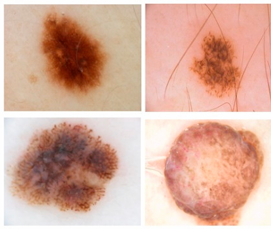
\includegraphics[width=0.75\textwidth]{3/figures/datapaper.png}
		\caption[Dataset usado en el artículo de \cite{karshiev2020improved}]{Dataset usado en el artículo de \cite{karshiev2020improved}.\\
		Fuente: \cite{karshiev2020improved}. \citetitle{karshiev2020improved}. (p. 2)}
		\label{3:fig2}
	\end{center}
\end{figure}

\begin{itemize}
    \item \textbf{Repositorios de Datasets de Imágenes Faciales}: Existen múltiples repositorios en línea dedicados específicamente a la recopilación y distribución de imágenes faciales. Plataformas como Kaggle, Papers with Code, y OpenML ofrecen conjuntos de datos etiquetados que incluyen rostros humanos con diferentes características morfológicas como arrugas, manchas, expresiones y edades. Estos datasets son fundamentales para el entrenamiento y evaluación de modelos de redes neuronales convolucionales, y suelen estar acompañados de documentación sobre su uso y licencia.
	\item \textbf{Bibliotecas Digitales y Bases de Datos Académicas}: Las bibliotecas digitales y bases de datos académicas también representan una fuente valiosa para obtener datasets faciales. En publicaciones académicas y tesis disponibles en plataformas como IEEE Xplore, SpringerLink, ScienceDirect y Google Scholar, es común encontrar referencias a datasets faciales utilizados en investigaciones previas. Estas fuentes permiten identificar conjuntos de datos validados por la comunidad científica y conocer sus aplicaciones en diferentes contextos, como el reconocimiento facial o el análisis de envejecimiento.
	\item \textbf{Plataformas de Código Abierto y Comunidades de Investigación}: Plataformas como GitHub, Hugging Face y Zenodo son ampliamente utilizadas por la comunidad investigadora para compartir datasets y modelos preentrenados. En estos repositorios, los investigadores publican conjuntos de imágenes faciales junto con scripts de preprocesamiento, anotaciones y arquitecturas de redes neuronales. Muchos de estos recursos se distribuyen bajo licencias abiertas (como CC BY o MIT).
  \end{itemize}


  %\newpage
\section{Técnicas para el procesamiento y análisis de la información}

\subsection{Metodología de implementación de la solución}

La creación de un Modelo de Segmentación Avanzada de Características Morfológicas varias fases de desarrollo, que van desde la recopilación de imágenes hasta su despliegue, como se menciona en el trabajo de \cite{yoon2023}. La imagen adquirida debe pasar por un proceso detallado posteriormente para alcanzar su etapa final. La metodología de esta investigación se muestra en la Figura \ref{3:fig3}.

\begin{figure}[h]
	\begin{center}
		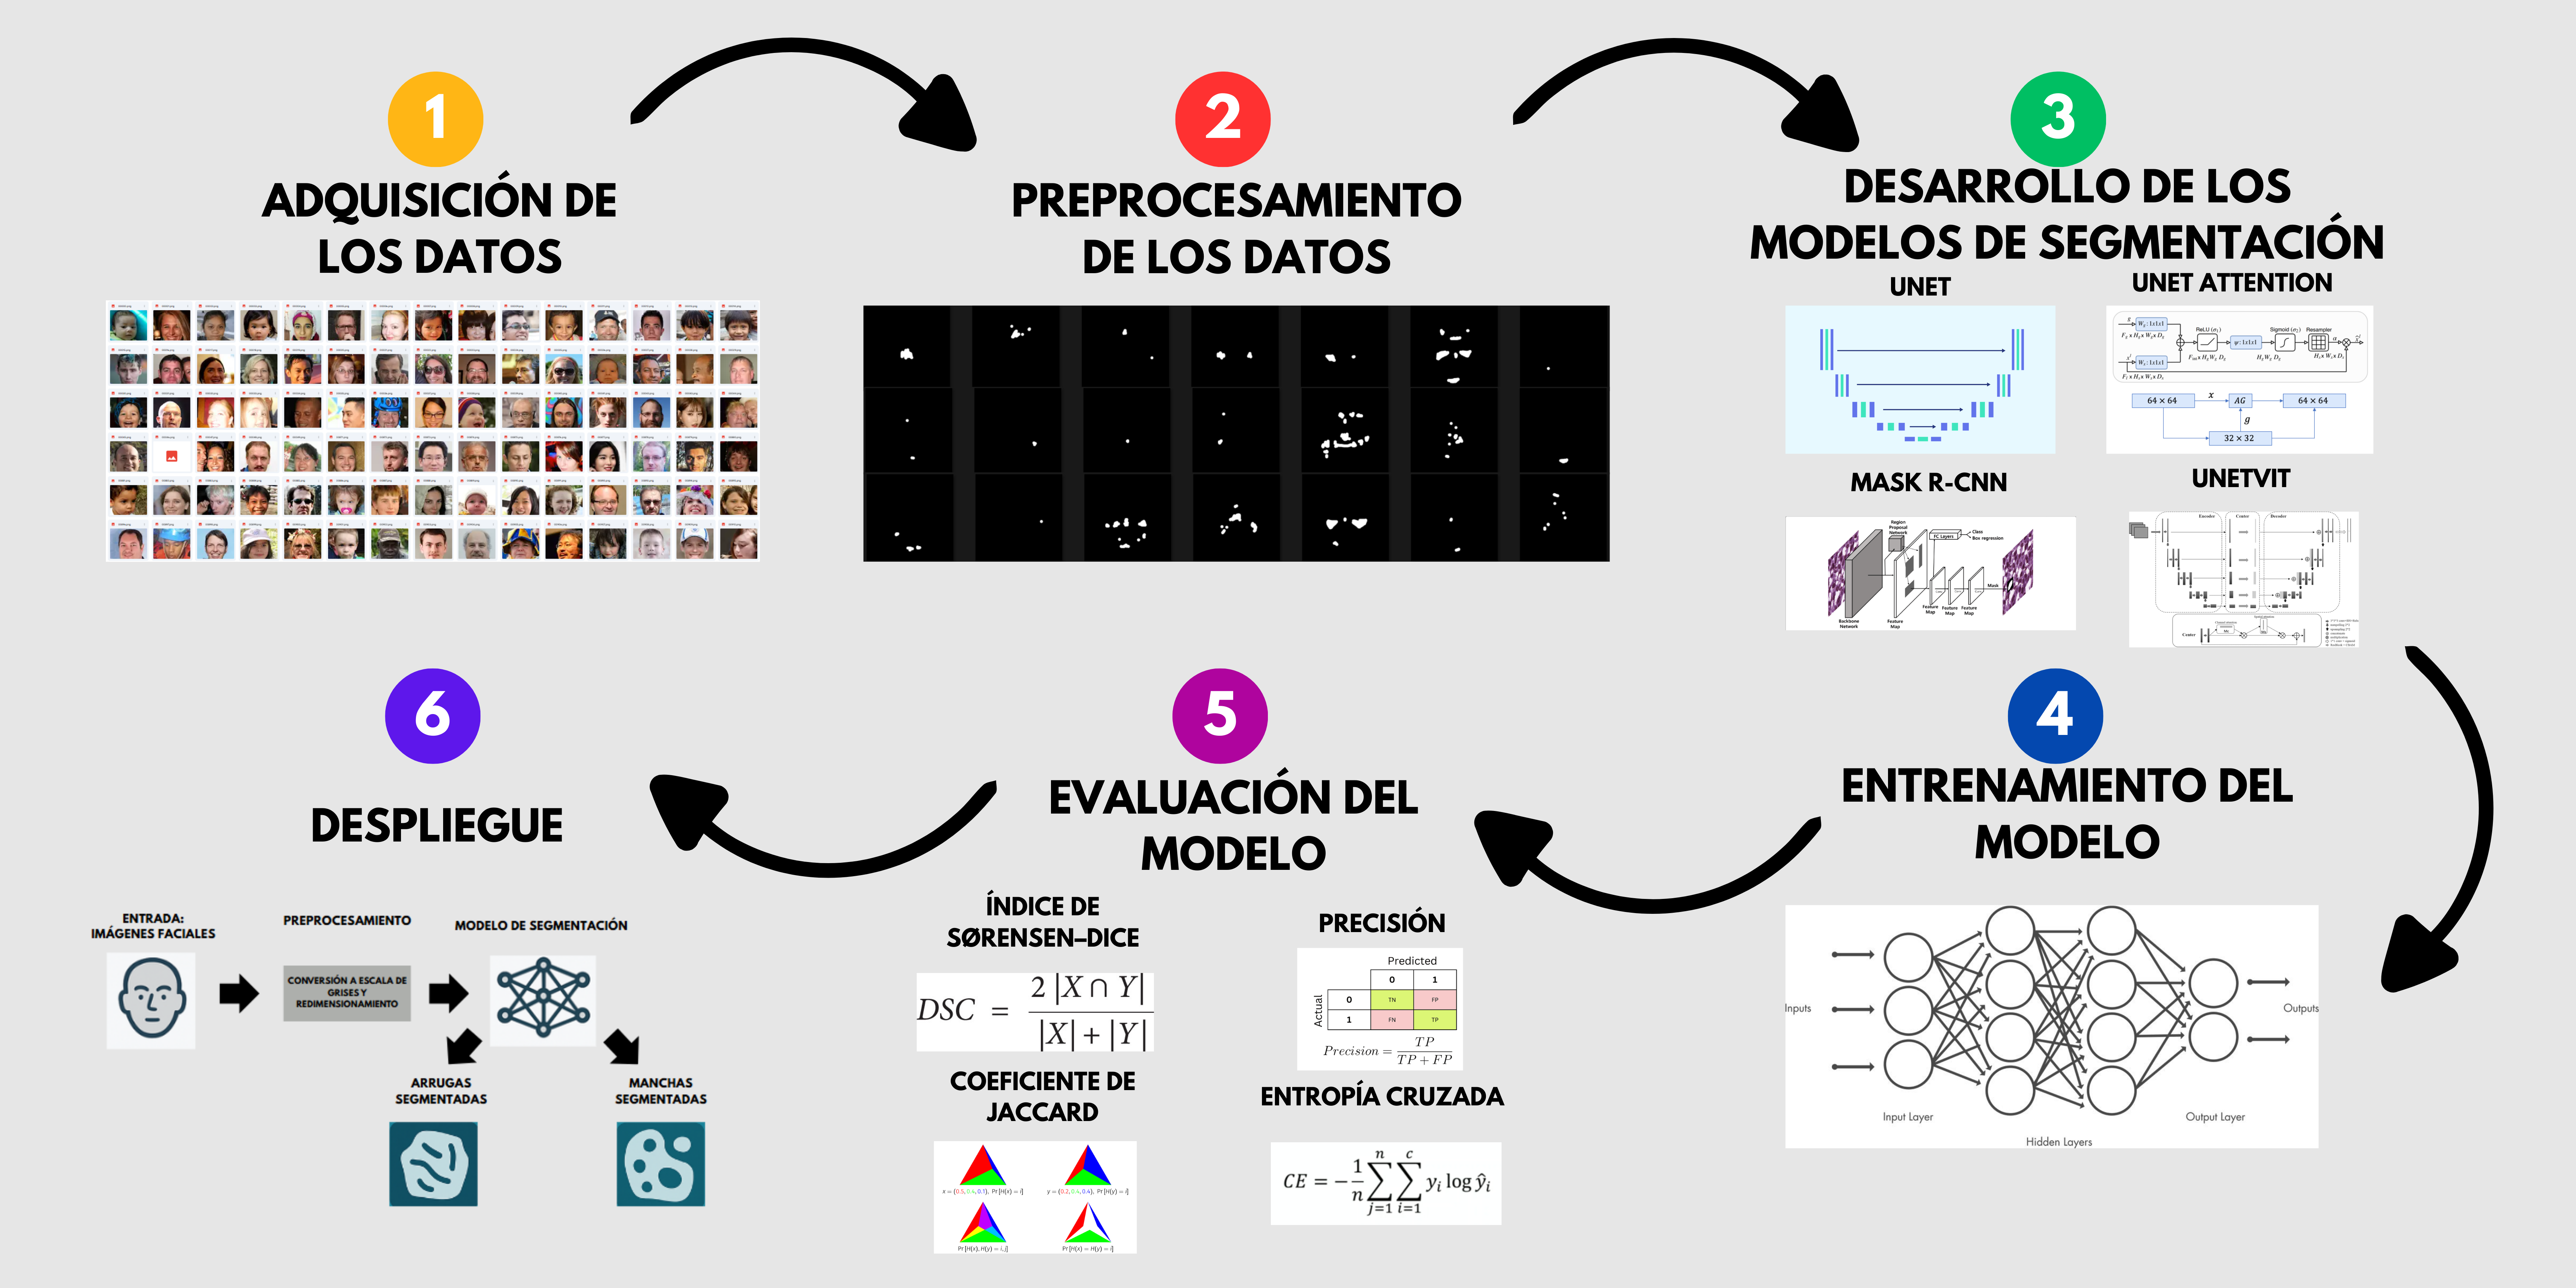
\includegraphics[width=1\textwidth]{3/figures/metodologia.png}
		\caption[Diagrama de Metodología de Investigación]{Diagrama de Metodología de Investigación.\\
			Fuente: Elaboración propia.}
		\label{3:fig3}
	\end{center}
\end{figure}


\subsubsection{Adquisición de los Datos}

En esta sección se describe el procedimiento utilizado para obtener el conjunto de datos empleado en este estudio. A continuación, se presenta una tabla que resume las tareas y actividades realizadas durante esta fase de adquisición. El primer paso fue la recopilación de datos. Los detalles sobre las actividades y tareas se encuentran en la Tabla \ref{tabla:actividades}.

Modelo ensamblado conceptualmente, listo para su implementación en entorno de desarrollo.

\subsubsection{Preprocesamiento de los Datos}
Se realizará el preprocesamiento de las imágenes del conjunto en esta etapa. La tabla \ref{tabla:preprocesamiento} incluye las tareas y actividades necesarias para completar la etapa de preprocesamiento:
\vspace{2ex}


\begin{longtable}{p{3cm}p{3cm}p{9cm}}
    \caption{Actividades de la fase de Preprocesamiento de Datos.}
    \label{tabla:preprocesamiento}\\
    \toprule
    \textbf{Actividades} & \textbf{Descripción} & \textbf{Tareas} \\
    \midrule
    \endfirsthead

    \toprule
    \textbf{Actividades} & \textbf{Descripción} & \textbf{Tareas} \\
    \midrule
    \endhead

    \bottomrule
    \endfoot

    \bottomrule
    \endlastfoot

    Filtración de imágenes faciales con características morfológicas & Eliminación de imágenes con baja resolución, mala iluminación o sin las características morfológicas de interés (arrugas y manchas), para mejorar la calidad del conjunto de datos. & 
    \begin{itemize}
        \item Eliminar imágenes borrosas, sobreexpuestas o subexpuestas.
        \item Conservar solo imágenes con resolución mínima de 128×128 píxeles.
        \item Seleccionar imágenes que contengan al menos una característica morfológica visible: arrugas o manchas.
        \item Verificar que el rostro esté completamente visible y centrado en la imagen.
    \end{itemize} \\

    Representación y normalización de las imágenes faciales & Conversión de las imágenes a formatos adecuados para su análisis por redes neuronales convolucionales. & 
    \begin{itemize}
        \item Redimensionar todas las imágenes a un tamaño uniforme.
        \item Convertir las imágenes a escala de grises o RGB, según el modelo.
        \item Normalizar los valores de píxeles entre 0 y 1.
        \item Aumentar los datos mediante técnicas como rotación, volteo, y zoom para mejorar la generalización.
    \end{itemize} \\

\end{longtable}

\begin{flushleft}
	\small Fuente: Elaboración propia.
\end{flushleft}

Enseguida, se describe en detalle las actividades junto con el resultado esperado.

\textbf{Actividad 1: Filtración de imágenes faciales con características morfológicas}
\\
En la fase de preprocesamiento de datos, la actividad de Filtración se enfoca en depurar y mejorar la calidad del conjunto de datos al eliminar información irrelevante o poco confiable. Esto se logra a través de la eliminación de datos no estándar y la conservación de aquellos que cumplen con criterios específicos de relevancia y fiabilidad. 

\textbf{Entregable}: Conjunto de datos filtrado y optimizado para su posterior análisis.

\textbf{Actividad 2: Representación y normalización de las imágenes faciales}
\\
Por otro lado, la actividad de Representación se encarga de convertir los datos en un formato visual o estructurado más adecuado para su análisis y comprensión. Esto implica transformar los datos en imágenes o representaciones gráficas que faciliten su visualización y entendimiento, contribuyendo así a una mejor interpretación por parte de los usuarios finales, como podemos observar en la Figura \ref{3:fig4}.

\textbf{Entregable}: Representación visual y estructurada de cada rostro facial en un formato adecuado para su procesamiento y análisis posterior.

\begin{figure}[h]
     \begin{center}
         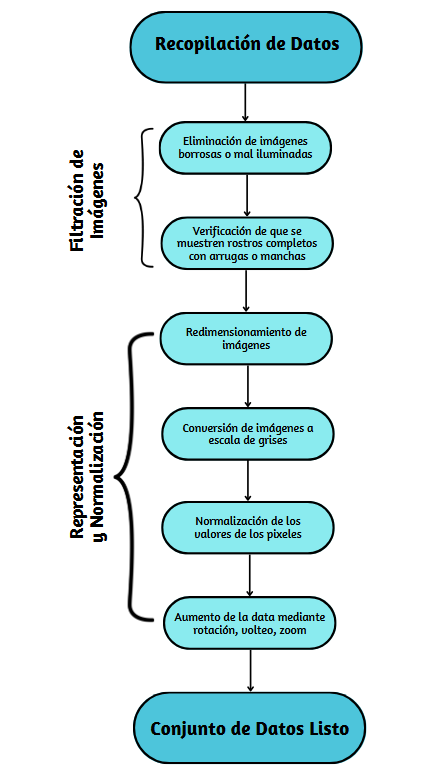
\includegraphics[width=0.8\textwidth]{3/figures/Diagrama de preprocesamiento.png}
         \caption[Diagrama de Preprocesamiento de los Datos]{Diagrama de Preprocesamiento de los Datos.\\
         Fuente: Elaboración propia}
         \label{3:fig4}
     \end{center}
 \end{figure}


 \subsubsection{Desarrollo de los Modelos de Segmentación}
 El desarrollo de los modelos de segmentación de características faciales se estructura en tres actividades clave. Estas actividades incluyen el diseño, implementación y entrenamiento de modelos basados en arquitecturas de redes neuronales profundas como U-Net, ResNet y modelos híbridos con Vision Transformer (ViT). La Tabla \ref{tabla:actividades_segmentacion} presenta el detalle de cada una.

 \vspace{2ex}
 \begingroup
 \renewcommand\arraystretch{1.2}
 \begin{longtable}{p{4cm} p{6cm} p{6cm}}
 \caption{Actividades de la fase de Desarrollo del Modelo de Segmentación.}
 \label{tabla:actividades_segmentacion}\\
 \toprule
 \textbf{Actividades} & \textbf{Descripción} & \textbf{Tareas} \\
 \midrule
 \endfirsthead
 
 \toprule
 \textbf{Actividades} & \textbf{Descripción} & \textbf{Tareas} \\
 \midrule
 \endhead
 
 \bottomrule
 \endfoot
 
 Diseño de la arquitectura del modelo & Selección conceptual y estructural de modelos apropiados para la segmentación de características morfológicas faciales. &
 \begin{itemize}
     \item Análisis de U-Net para segmentación precisa de áreas pequeñas como arrugas y poros.
     \item Evaluación del potencial de ResNet para representar características profundas y complejas.
     \item Consideración de arquitecturas híbridas que integren CNN con Vision Transformer (ViT).
 \end{itemize} \\
 
 Definición de componentes del modelo & Establecimiento de las partes esenciales del modelo para la segmentación de imágenes faciales. &
 \begin{itemize}
     \item Diseño de capas convolucionales, de codificación y decodificación.
     \item Propuesta de bloques residuales y mecanismos de atención en modelos híbridos.
     \item Configuración de dimensiones de entrada y salida adaptadas a imágenes faciales.
 \end{itemize} \\
 
 Estrategia de ensamblado del modelo & Organización lógica y estructural de los bloques que conforman cada arquitectura seleccionada. &
 \begin{itemize}
     \item Integración de módulos especializados según la arquitectura (por ejemplo, skip connections en U-Net).
     \item Planificación de rutas de información para mejorar la segmentación espacial.
     \item Definición de la estructura jerárquica de procesamiento de la imagen.
 \end{itemize} \\
 
 \end{longtable}
 \endgroup

 Enseguida, se proporciona en la Figura \ref{3:fig5} el diagrama de cada actividad, y a su vez un detalle de la actividad junto con el entregable correspondiente que se espera obtener.
 
 \textbf{Actividad 1: Diseño de la arquitectura del modelo}
 \\
 Durante esta etapa se define la estructura general de las redes neuronales que se utilizarán para la segmentación de características morfológicas faciales. El objetivo es seleccionar arquitecturas que sean adecuadas para extraer información precisa de regiones faciales como arrugas, poros o manchas.
 Entre las arquitecturas consideradas se encuentra U-Net, que destaca por su capacidad de segmentación precisa gracias a su estructura simétrica y sus conexiones de salto entre el codificador y el decodificador. También se evalúa el uso de ResNet, una arquitectura que incorpora bloques residuales para mejorar el aprendizaje en redes profundas, especialmente útil para capturar texturas complejas. Asimismo, se contempla la exploración de modelos híbridos que combinan Redes Neuronales Convolucionales (CNN) con Vision Transformer (ViT), lo cual permite captar patrones sutiles mediante mecanismos de atención.
 
 \textbf{Entregable}: Selección de la arquitectura óptima para el modelo de segmentación facial, justificada técnicamente.

 \textbf{Actividad 2: Definición de componentes del modelo}
 \\
Esta actividad consiste en establecer los elementos esenciales que conformarán las redes previamente seleccionadas. Se determina la cantidad de capas, el tipo de operaciones dentro de cada módulo y la forma en que se conectan entre sí, en función de las necesidades de segmentación facial.

En U-Net, por ejemplo, se define cuántas capas de codificación y decodificación se utilizarán, así como las conexiones que transmitirán información detallada entre estas. En ResNet, se especifica el número de bloques residuales y la profundidad de la red, asegurando que se mantenga la eficiencia del aprendizaje sin perder información relevante. En los modelos híbridos con ViT, se determina cómo integrar los módulos de atención con las capas convolucionales, de forma que se mantenga un flujo eficiente de características entre ambos entornos.

 \textbf{Entregable}: Especificación detallada de los componentes y estructura interna de cada arquitectura seleccionada.


 \textbf{Actividad 3: Estrategia de ensamblado del modelo}
 \\
 La última actividad del desarrollo se enfoca en ensamblar los componentes definidos en una arquitectura operativa y coherente. El ensamblado implica organizar los módulos en un orden lógico que permita un flujo fluido de datos desde la entrada hasta la salida del modelo.

Para U-Net, esto implica establecer correctamente las conexiones tipo “skip” que permiten recuperar detalles espaciales perdidos durante la codificación. En el caso de ResNet, se ensamblan los bloques residuales de forma que la información pueda circular libremente entre capas profundas. Finalmente, para los modelos híbridos, se debe asegurar que las características extraídas por las CNN puedan ser procesadas adecuadamente por los módulos de atención del Vision Transformer, logrando así una representación enriquecida para la segmentación facial.

 \textbf{Entregable}: Modelo ensamblado conceptualmente, listo para su implementación en entorno de desarrollo.

 
 \begin{figure}[h]
    \begin{center}
        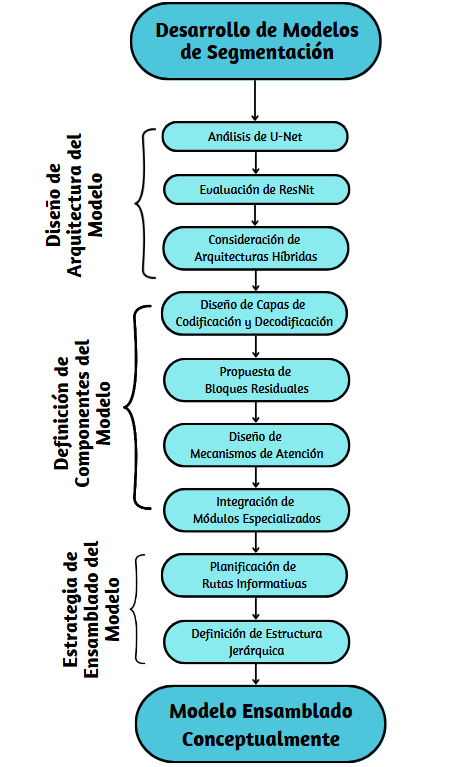
\includegraphics[width=0.8\textwidth]{3/figures/Diagrama de Desarrollo.png}
        \caption[Diagrama del Desarrollo de los Modelos de Segmentación]{Diagrama del Desarrollo de los Modelos de Segmentación.\\
        Fuente: Elaboración propia}
        \label{3:fig5}
    \end{center}
\end{figure}

\subsubsection{Entrenamiento del Modelo}
Al concluir la etapa de Desarrollo de Modelos de Segmentación, se continua con el Entrenamiento, en la Tabla \ref{tabla:entrenamiento_modelo} fue diseñada siguiendo las actividades.

\vspace{2ex}
 \begingroup
 \renewcommand\arraystretch{1.2}
 \begin{longtable}{p{4cm} p{6cm} p{6cm}}
 \caption{Actividades de la fase de Entrenamiento del Modelo.}
 \label{tabla:entrenamiento_modelo}\\
 \toprule
 \textbf{Actividades} & \textbf{Descripción} & \textbf{Tareas} \\
 \midrule
 \endfirsthead
 
 \toprule
 \textbf{Actividades} & \textbf{Descripción} & \textbf{Tareas} \\
 \midrule
 \endhead
 
 \bottomrule
 \endfoot
 
 Configuración del entorno de entrenamiento &
 Preparación del entorno computacional y los recursos necesarios para el entrenamiento del modelo. &
 \begin{itemize}
     \item Selección del framework (TensorFlow o PyTorch).
     \item Habilitación del uso de GPU para acelerar el entrenamiento.
     \item Establecimiento de rutas de acceso a los datos y modelos.
 \end{itemize} \\
 
 Aplicación de técnicas de optimización &
 Utilización de métodos que permitan una mejora progresiva del modelo a lo largo de las épocas de entrenamiento. &
 \begin{itemize}
     \item Configuración del optimizador Adam para minimizar la función de pérdida.
     \item Ajuste de tasa de aprendizaje, tamaño de batch y número de épocas.
     \item Monitorización de la evolución del \textit{loss} y métricas de precisión.
 \end{itemize} \\
 
 Validación cruzada del rendimiento &
 Evaluación del desempeño del modelo utilizando múltiples divisiones del conjunto de datos. &
 \begin{itemize}
     \item División del dataset en k pliegues para pruebas y entrenamiento.
     \item Entrenamiento del modelo en diferentes subconjuntos.
     \item Análisis del promedio de métricas obtenidas para garantizar estabilidad.
 \end{itemize} \\
 
 \end{longtable}
 \endgroup

\subsubsection{Evaluación del Modelo}
El desempeño del sistema de segmentación será evaluado utilizando métricas específicas para problemas de clasificación y segmentación:
\begin{itemize}
    \item \textbf{Precisión (Accuracy):} Proporción de predicciones correctas sobre el total de predicciones.
    \item \textbf{Recall (Sensibilidad):} Proporción de características positivas correctamente identificadas.
    \item \textbf{F1-Score:} Promedio armónico de precisión y recall, útil para conjuntos de datos desbalanceados.
    \item \textbf{AUC-ROC:} Área bajo la curva ROC para medir la capacidad del modelo de distinguir entre clases.
\end{itemize}

Adicionalmente, se utilizará una matriz de confusión para analizar en detalle los errores cometidos por los modelos, lo que permitirá identificar patrones en los casos mal clasificados.

\subsubsection{Despliegue}
El modelo seleccionado será integrado en un prototipo funcional que permitirá procesar imágenes faciales y generar un reporte detallado de las características segmentadas. Este prototipo incluirá una interfaz amigable que mostrará:
\begin{itemize}
    \item Mapas de calor que destacarán áreas con arrugas, poros dilatados y manchas.
    \item Gráficos comparativos que mostrarán la evolución de las características morfológicas.
    \item Recomendaciones personalizadas basadas en el análisis segmentado.
\end{itemize}

Las pruebas finales se realizarán en un entorno simulado para verificar su rendimiento en casos prácticos, como evaluaciones estéticas en clínicas dermatológicas o la personalización de tratamientos cosméticos.

\section{Metodología para la Medición de Resultados de la Implementación}

Para garantizar la correcta evaluación del sistema, se emplearán las siguientes métricas basadas en la matriz de confusión:
\begin{itemize}
    \item \textbf{Precisión (Accuracy):} \[ accuracy = \frac{TP + TN}{TP + TN + FP + FN} \]
    \item \textbf{Recall:} \[ recall = \frac{TP}{TP + FN} \]
    \item \textbf{Precisión Positiva:} \[ precision = \frac{TP}{TP + FP} \]
    \item \textbf{F1-Score:} \[ F1 = 2 \cdot \frac{precision \cdot recall}{precision + recall} \]
\end{itemize}

Cada métrica será calculada para determinar la efectividad del modelo en la segmentación de arrugas, poros y manchas, evaluando su capacidad de proporcionar predicciones precisas y consistentes en datos no vistos.
%%%%%%%%%%%%%%%%%%%%%%%%%%%%%%%%%%%%%%

\begin{landscape}
	\section{Cronograma de actividades y presupuesto}
	Se propuso un cronograma para la investigación. Conforma desde el inicio hasta ser terminada con la sustentación final planeada para mediados del año 2024. Este se presneta en la Figura \ref{3:fig303}.

	\begin{figure}[!ht]
		\begin{center}
			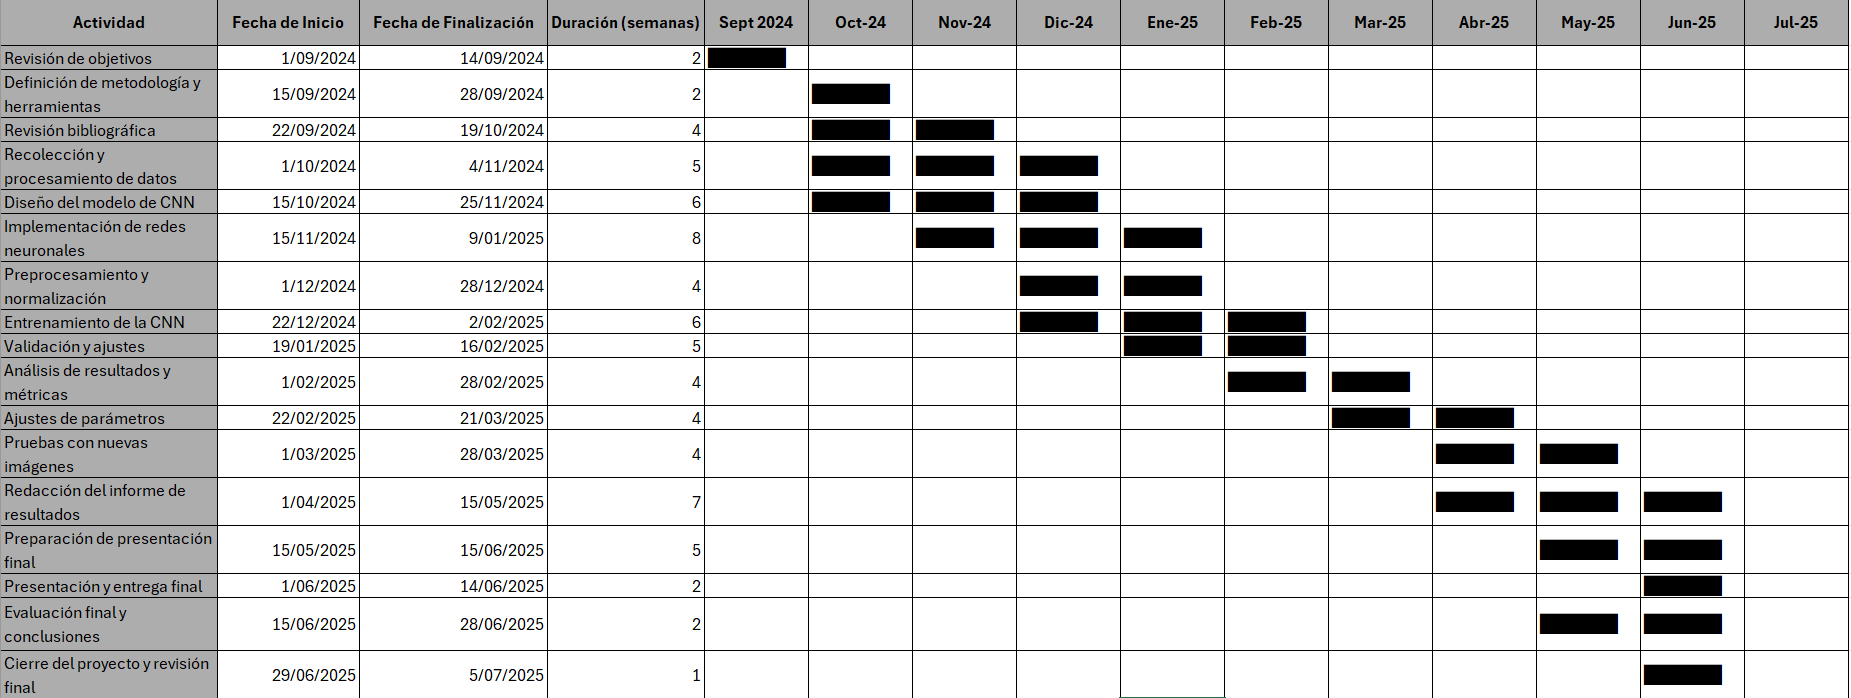
\includegraphics[width=1.50\textwidth]{3/figures/gant.png}
			\caption[Cronograma de actividades]{Cronograma de actividades.\\
				Fuente: Elaboración propia.}
			\label{3:fig303}
		\end{center}
	\end{figure}
	
\end{landscape}
%%%%%%%%%%%%%%%%%%%%%%%%%%%%%%%%%%%%%%%%

%%%%%%%%%%%%%%%%%%%%%%%%%%%%%%%




Se determinó el siguiente presupuesto necesario para la elaboración completa de la investigación. Este se presenta en la Tabla \ref{3:table1}.

\begin{table}[H]
	\caption[Presupuesto]{Presupuesto estimado para el desarrollo del sistema de segmentación morfológica.}
	\label{3:table1}
	\centering
	\small
	\begin{tabular}{llll}
		\specialrule{.1em}{.05em}{.05em}
		{Grupo} & {Item} & {Costo (soles)} & {Subtotal} \\ 
		\specialrule{.1em}{.05em}{.05em}
		\multirow{3}{4cm}{Recursos materiales} 
		& {Laptop de alto rendimiento} & {S/ 7,500.00} & {} \\ 
		& {Materiales de escritorio} & {S/ 150.00} & {} \\
		& {Dispositivo de almacenamiento externo} & {S/ 300.00} & {S/ 7,950.00} \\ 
		\cline{1-4}
		\multirow{3}{4cm}{Software y servicios} 
		& {Licencia de software (Python/IDE)} & {S/ 50.00} & {} \\
		& {Renta de servidor en la nube} & {S/ 500.00} & {} \\
		& {Acceso a bases de datos de imágenes} & {S/ 300.00} & {S/ 850.00} \\ 
		\cline{1-4}
		\multirow{3}{4cm}{Costos académicos} 
		& {Matrícula en Trabajo de Tesis II} & {S/ 375.00} & {} \\
		& {Cuotas de Trabajo de Tesis II} & {S/ 1,044.00} & {S/ 1,419.00} \\ 
		\cline{1-4}
		\multirow{2}{4cm}{Extras} 
		& {Consultorías especializadas} & {S/ 200.00} & {} \\
		& {Movilidad y transporte} & {S/ 300.00} & {S/ 500.00} \\ 
		\specialrule{.1em}{.05em}{.05em} 
		{} & {Total} & {} & {S/ 10,719.00} \\ 
		\specialrule{.1em}{.05em}{.05em}
	\end{tabular}
	\begin{flushleft}	
		\small Fuente: Elaboración propia.
	\end{flushleft}
\end{table}




